\chapter{Results}
\label{chap5}
\setlength{\tabcolsep}{5pt}
In this chapter we approximate an artificial Rayleigh integral.
The settings to synthetically construct the integral are listed in Section \ref{settings}, and the integrand is displayed in Figure \ref{fig:projected_wavefield}.
Table \ref{tab:single} contains performance data of the evaluation of a single integral, whereas Table \ref{tab:average} contains averaged data of the computation of multiple integrals.
We compare various methods to approximate the integral in Section \ref{res_discussion} (the methods are listed in Section \ref{summary_used_method}).
Also, the computer code used to generate these results can be found in Appendix \ref{app:code}.

\section{Settings}
\label{settings}
The settings used for generating the results and constructing the artificial integral are as follows:
\begin{itemize}
    \itemsep0pt
    \item We integrate on the interval $[-25, 25] \times [-35, 35]$, the integrand can be seen in Figure \ref{fig:projected_wavefield}.
    \item To simulate a wavefield we used multiple sources placed at $(x_s, y_s, z_s) = (10, 0, 2)$, $(0, 15, 1.5)$, $(1, -5, 1.7)$ and $(-13, 13, 2.3)$.
    \item In all results we used $k=\omega / c = 2 \pi / \lambda = 0.5$, thus $\lambda = 4 \pi$ (note that $\lambda$ denotes wavelength).
    \item In Table \ref{tab:single} we used a prediction point located at $(x_A, y_A, z_A) = (0.9, -1.4, -10)$, in Table \ref{tab:average} we used multiple prediction points located at $(x_A, y_A, z_A) = (0.9, -1.4, 10)$, $(2, -1, 9)$, $(-1, 2, 11)$, $(-3, 4, 11.5)$, $(0.1, 1.4, 9.5)$, $(0.5, -1.5, 10)$, $(2.1, -1.1, 9)$, $(-1.1, 2.1, 11)$, $(-3.1, 4.1, 11.5)$, and $(0.2, 1.5, 9.5)$. The motivation to use multiple prediction points and average them was that the generated table (Table \ref{tab:single}) has coincidences where the calculated integral is really close to the actual integral because deflections cancelled each other (thus a method could get lucky and have a better result than a method that is better in general), taking an average ironed (some of) these coincidences out.
    \item We calculated the points per wavelength from the number of sample points, the following numbers of sample points were used: $(\textrm{samples}_x, \textrm{samples}_y) =$ (19, 9), (29, 29), (49, 49), (69, 69), (99, 99), (199, 199) and (499, 499), respectively. We then used the following formula (dependent on direction) to calculate the points per wavelength (note that we let $i$ denote the direction and $h_i$ the width of the interval in that direction):
        \begin{equation}
            (\textrm{points} / \lambda)_i = \frac{\lambda (\textrm{samples}_i - 1)}{h_i} \,. \nonumber
        \end{equation}
\end{itemize}

\section{Discussion}
\label{res_discussion}
Upon inspecting Figure \ref{fig:samplesa} with approximately 1.44 points per wavelength we can see that there is no hope left to approximate the integral.
Whereas using approximately 5 sample points per wavelength in Figure \ref{fig:samplesb} seems doable, resulting in relatively close integrals (see Table \ref{tab:single} and Table \ref{tab:average}).
\begin{figure}[H]
    \centering
    \begin{tabular}{cc}
        \subcaptionbox{\centering Real part of $P \nabla G$ (the integrand) \label{fig:real_3d_projected_wavefield}}{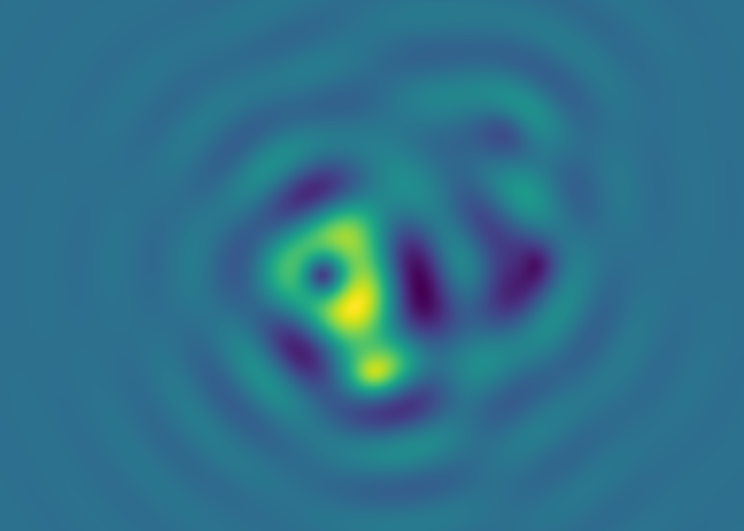
\includegraphics[width=.47\textwidth]{pictures/real_3d_part_projected}} &
        \subcaptionbox{\centering Imaginary part of $P \nabla G$ (the integrand) \label{fig:proj_b}}{
\includegraphics[width=.47\textwidth]{pictures/imag_3d_part_projected}} \\
        \subcaptionbox{\centering Real part of $P \nabla G$ (the integrand) at $x=0$ \label{fig:proj_c}}{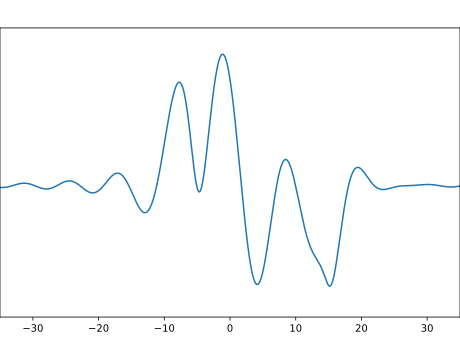
\includegraphics[width=.47\textwidth]{pictures/real_2d_part}} &
        \subcaptionbox{\centering Imaginary part of $P \nabla G$ (the integrand) at $x=0$ \label{fig:proj_d}}{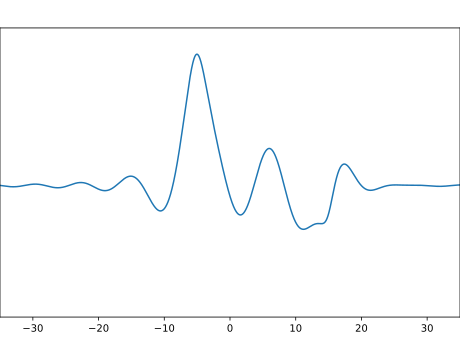
\includegraphics[width=.47\textwidth]{pictures/imag_2d_part}}
    \end{tabular}
    \caption{The integrand of the artificial Rayleigh integral for a prediction point at $(x_A, y_A, z_A) = (0.9, -1.4, -10)$ and sources at locations described in Section \ref{settings}. The Figures (a) and (b) are rotated such that the $y$-direction is horizontal and the $x$-direction is vertical. The Figures (c) and (d) can be extracted from Figures (a) and (b) by looking at the intensity of the wavefield in the middle, horizontal line (where $x=0$).}
    \label{fig:projected_wavefield}
\end{figure}
\begin{figure}[H]
    \vspace{-2em}
    \centering
    \begin{tabular}{cc}
        \subcaptionbox{\centering Real part of $P \nabla G$ (the integrand) at $x=0$ with 9 sample points, i.e. approximately 1.44 sample points per wavelength. \label{fig:samplesa}}{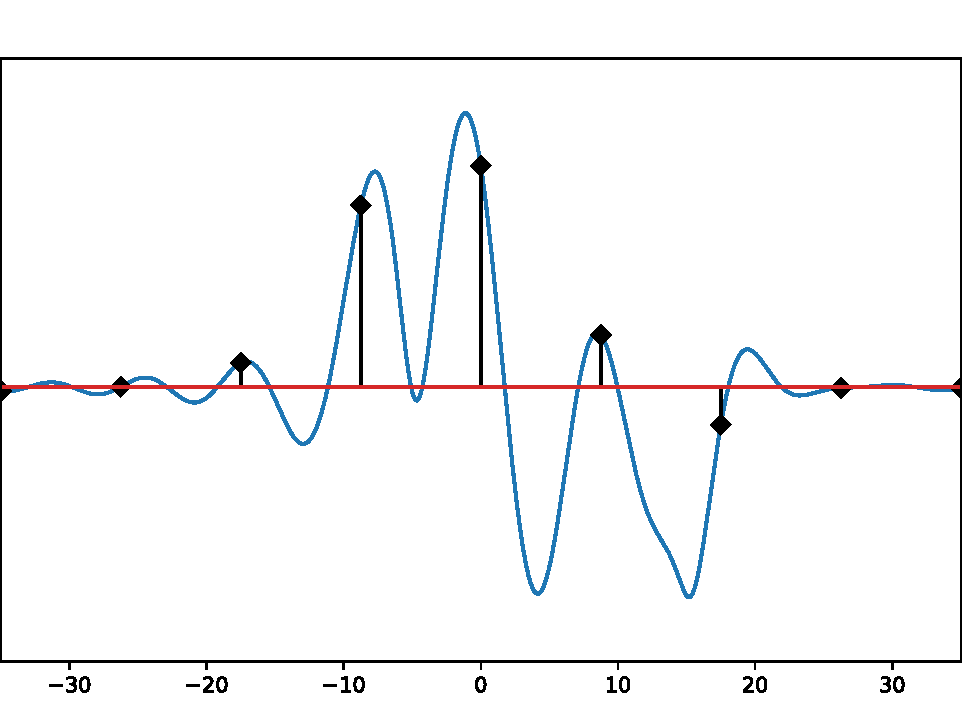
\includegraphics[width=.47\textwidth]{pictures/samples_19_9}} &
        \subcaptionbox{\centering Real part of $P \nabla G$ (the integrand) at $x=0$ with 29 sample points, i.e. approximately 5.03 sample points per wavelength.\label{fig:samplesb}}{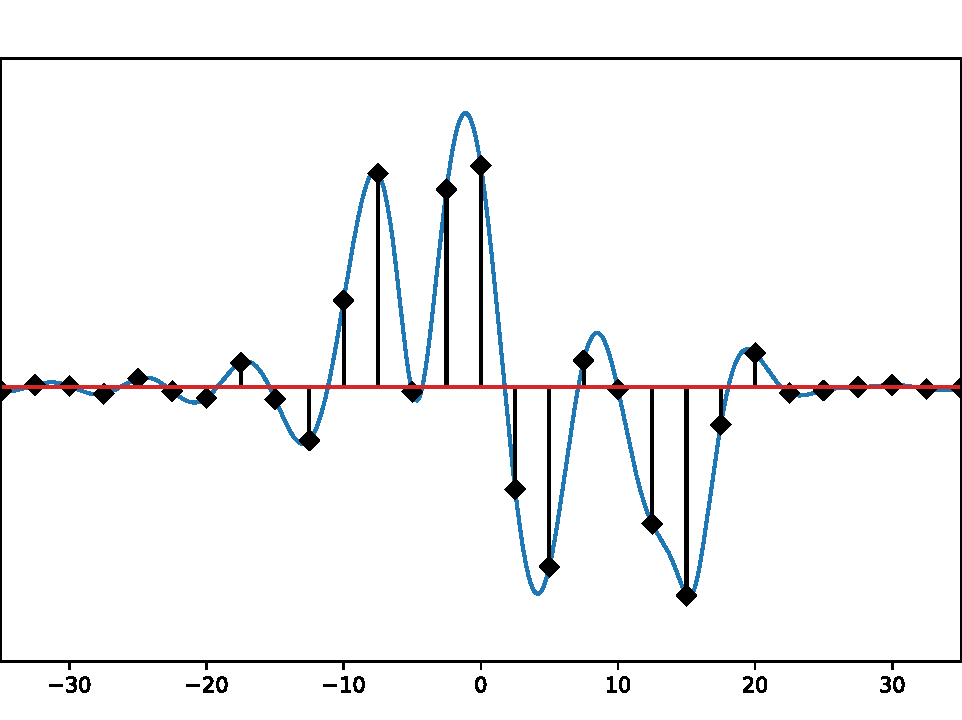
\includegraphics[width=.47\textwidth]{pictures/samples_29_29}}
        % \subcaptionbox{\centering Real part of $P \nabla G$ (the integrand) at $x=0$ with 49 sample points, i.e. approximately 8.62 sample points per wavelength.\label{fig:samplesc}}{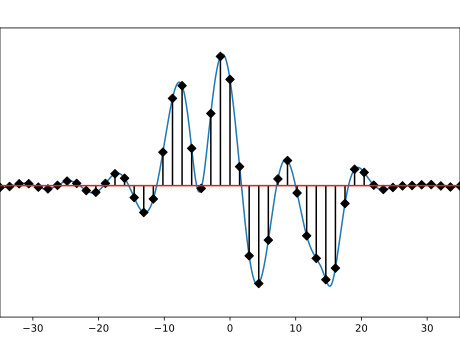
\includegraphics[width=.47\textwidth]{pictures/samples_49_49}} &
        % \subcaptionbox{\centering Real part of $P \nabla G$ (the integrand) at $x=0$ with 69 sample points, i.e. approximately 12.2 sample points per wavelength.\label{fig:samplesd}}{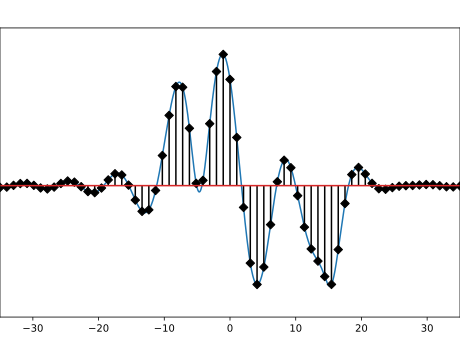
\includegraphics[width=.47\textwidth]{pictures/samples_69_69}}
    \end{tabular}
    \caption{Figure \ref{fig:proj_c}, displayed with varying amounts of sample points (per wavelength).}
\end{figure}

% Noise = 0.2\%, Max noise = 0.9\% for 500, Av noise = 0.16\%
\begin{table}[H]
\centering
    \begin{tabular}{|c|c|ccccccc|}
        \hline
        \multirow{2}{*}{Noise} & (points/$\lambda$)$_x$ & 4.52 & 7.04 & 12.1 & 17.1 & 24.6 & 49.8 & 125 \\
        & (points/$\lambda$)$_y$ & 1.44 & 5.03 & 8.62 & 12.2 & 17.6 & 35.5 & 89.4 \\
        % \multirow{2}{*}{Noise} & samples$_x$ & 19 & 29 & 49 & 69 & 99 & 199 & 499 \\
        % & samples$_y$ & 9 & 29 & 49 & 69 & 99 & 199 & 499 \\
        \hline
        \hline
        \rowcolor[gray]{.9}
        \cellcolor{white}
        & basic & 1.5 & 6.6$\cdot 10^{-3}$ & 1.1$\cdot 10^{-3}$ & 5.5$\cdot 10^{-4}$ & 2.7$\cdot 10^{-4}$ & 6.5$\cdot 10^{-5}$ & 1.0$\cdot 10^{-5 }$ \\
        \cline{2-9}
        \cellcolor{white}
        & combined & 1.60 & 0.305 & 0.298 & 0.827 & 7.06 & 406. & 63.5 \\
        \cellcolor{white}
        \multirow{-3}{*}{0\%}& separate & 1.03 & 1.88 & 4.21 & 28.0 & 44.8 & 183. & 1.14$\cdot 10^{3}$ \\
        \hline
        \hline
        \rowcolor[gray]{.9}
        \cellcolor{white}
        & basic & 1.5 & 6.6$\cdot 10^{-3}$ & 1.1$\cdot 10^{-3}$ & 4.7$\cdot 10^{-4}$ & 2.5$\cdot 10^{-4}$ & 6.0$\cdot10^{-5}$ & 1.0$\cdot 10^{-5 }$ \\
        \cline{2-9}
        \cellcolor{white}
        & basic$_\delta$ & 1.00 & 1.01 & 1.03 & 0.864 & 0.942 & 0.920 & 1.01 \\
        \cellcolor{white}
        & combined & 1.60 & 0.302 & 0.311 & 0.696 & 5.06 & 15.7 & 11.5 \\
        \cellcolor{white}
        & combined$_\delta$ & 1.60 & 0.301 & 0.322 & 0.638 & 3.65 & 46.2 & 3.71 \\
        \cellcolor{white}
        & separate & 1.03 & 1.89 & 5.05 & 17.4 & 20.8 & 8.82 & 16.4 \\
        \cellcolor{white}
        \multirow{-6}{*}{0.05\%}
        & separate$_\delta$ & 1.02 & 1.88 & 4.42 & 25.1 & 49.4 & 282. & 356. \\
        \hline
        \hline
        \rowcolor[gray]{.9}
        \cellcolor{white}
        & basic & 1.5 & 6.6$\cdot 10^{-3}$ & 1.3$\cdot 10^{-3}$ & 2.5$\cdot 10^{-4}$ & 2.0$\cdot 10^{-4}$ & 4.7$\cdot 10^{-5}$ & 1.1$\cdot 10^{-5 }$ \\
        \cline{2-9}
        \cellcolor{white}
        & basic$_\delta$ & 0.999 & 1.05 & 1.13 & 0.458 & 0.771 & 0.698 & 1.07 \\
        \cellcolor{white}
        & combined & 1.60 & 0.296 & 0.348 & 0.306 & 1.56 & 3.16 & 3.29 \\
        \cellcolor{white}
        & combined$_\delta$ & 1.61 & 0.296 & 0.404 & 0.242 & 1.25 & 9.89 & 0.996 \\
        \cellcolor{white}
        & separate & 1.02 & 1.90 & 7.32 & 1.77 & 4.72 & 1.76 & 4.29 \\
        \cellcolor{white}
        \multirow{-6}{*}{0.2\%}
        & separate$_\delta$ & 1.02 & 1.89 & 5.04 & 14.9 & 65.1 & 89.4 & 81.2 \\
        \hline
        \hline
        \rowcolor[gray]{.9}
        \cellcolor{white}
        & basic & 1.5 & 8.4$\cdot 10^{-3}$ & 2.1$\cdot 10^{-3}$ & 1.0$\cdot 10^{-3}$ & 1.6$\cdot 10^{-4}$ & 6.4$\cdot 10^{-5}$ & 2.1$\cdot 10^{-5 }$ \\
        \cline{2-9}
        \cellcolor{white}
        & basic$_\delta$ & 0.995 & 1.60 & 1.51 & 2.06 & 0.764 & 0.712 & 1.76 \\
        \cellcolor{white}
        & combined & 1.62 & 0.343 & 0.518 & 0.464 & 0.271 & 0.861 & 1.32 \\
        \cellcolor{white}
        & combined$_\delta$ & 1.64 & 0.339 & 1.36 & 0.361 & 0.251 & 2.79 & 0.390 \\
        \cellcolor{white}
        & separate & 1.01 & 1.67 & 2.75 & 1.36 & 0.783 & 0.479 & 1.69 \\
        \cellcolor{white}
        \multirow{-6}{*}{1\%}
        & separate$_\delta$ & 1.00 & 2.44 & 8.50 & 105. & 11.7 & 19.4 & 33.0 \\
        \hline
        \hline
        \rowcolor[gray]{.9}
        \cellcolor{white}
        & basic & 1.2 & 3.0$\cdot 10^{-2}$ & 6.2$\cdot 10^{-3}$ & 7.3$\cdot 10^{-3}$ & 1.6$\cdot 10^{-3}$ & 5.0$\cdot 10^{-4}$ & 9.4$\cdot 10^{-5 }$ \\
        \cline{2-9}
        \cellcolor{white}
        & basic$_\delta$ & 0.967 & 2.17 & 2.91 & 10.0 & 3.38 & 0.933 & 0.593 \\
        \cellcolor{white}
        & combined & 1.80 & 0.798 & 0.864 & 0.707 & 0.542 & 1.34 & 1.18 \\
        \cellcolor{white}
        & combined$_\delta$ & 1.90 & 0.788 & 0.900 & 0.587 & 0.507 & 4.38 & 0.333 \\
        \cellcolor{white}
        & separate & 0.925 & 1.46 & 1.39 & 1.94 & 1.60 & 0.754 & 1.54 \\
        \multirow{-6}{*}{5\%}
        \cellcolor{white}
        & separate$_\delta$ & 0.818 & 7.85 & 54.6 & 123. & 27.8 & 46.5 & 48.0 \\
        \hline
        \hline
        \rowcolor[gray]{.9}
        \cellcolor{white}
        & basic & 7.5$\cdot 10^{-2}$ & 1.3$\cdot 10^{-1}$ & 1.9$\cdot 10^{-2}$ & 3.0$\cdot 10^{-2}$ & 7.1$\cdot 10^{-3}$ & 2.2$\cdot 10^{-3}$ & 3.7$\cdot 10^{-4 }$ \\
        \cline{2-9}
        \cellcolor{white}
        & basic$_\delta$ & 0.548 & 1.40 & 1.56 & 3.70 & 0.898 & 0.302 & 0.147 \\
        \cellcolor{white}
        & combined & 0.129 & 1.19 & 1.11 & 0.765 & 0.588 & 1.40 & 1.18 \\
        \cellcolor{white}
        & combined$_\delta$ & 0.117 & 1.53 & 0.545 & 0.560 & 0.538 & 0.659 & 0.174 \\
        \cellcolor{white}
        & separate & 0.109 & 1.58 & 1.06 & 2.21 & 1.90 & 0.818 & 1.71 \\
        \cellcolor{white}
        \multirow{-6}{*}{20\%}
        & separate$_\delta$ & 0.0474 & 12.4 & 37.9 & 43.6 & 33.5 & 265. & 128. \\
        \hline
    \end{tabular}
    \caption{For different amounts of noise (normal distributed, with a standard deviation of 0\%, 0.05\%, 0.2\%, 1\%, 5\% and 20\% of the length between equidistant points) and different amounts of samples points per wavelength varying per direction ((4.52, 1.44), (7.04, 5.03), (12.1, 8.62), (17.1, 12.2), (24.6, 17.6), (49.8, 35.5), (125, 89.4)) we listed the relative error (the mean-squared error was used due to working with complex numbers) of the approximation of the simulated Rayleigh integral (with settings listed in Section \ref{settings}) using the basic method described in Section \ref{summary_used_method}.
    Also, the other methods described in Section \ref{summary_used_method} are listed (where the adapted version of the method on a non-equidistant grid is denoted with a subscript $\delta$) with their relative error, divided by the relative error of the basic method.
    We thus have that the numbers represent the number of times that the used method is better than the basic method.
    We note that for a noise of 0\% the adapted versions of each method are the same as the regular methods, since we have no uncertainty in gridpoints.
    Furthermore, to give an example: for a noise of 0.2\% (thus each gridpoints is shifted in the $x$-direction with $\mathcal N(0.2\% \cdot h_x)$ and in the $y$-direction with $\mathcal N(0.2\% \cdot h_y)$, where $h_x$, $h_y$ denote the distance between the equidistant gridpoints in the $x$ and $y$-directions respectively and $\mathcal N(\sigma)$ denotes normal distributed noise with standard deviation $\sigma$) and 12.1 samples per wavelength in the $x$-direction and $8.62$ samples per wavelength in the $y$-direction, the basic method has a relative error of $1.3\cdot 10^{-3}$, whereas the altered separate method (separate$_\delta$) has a relative error that is $5.04$ times as low, i.e. $1.3/5.04\cdot 10^{-3} \approx 2.6\cdot 10^{-4}$ and the combined method has a relative error that is larger than the error of the basic method with a factor of $1/0.348 \approx 2.87$.}
    \label{tab:single}
\end{table}


\begin{table}[H]
\centering
    \begin{tabular}{|c|c|ccccccc|}
        \hline
        \multirow{2}{*}{Noise} & (points/$\lambda$)$_x$ & 4.52 & 7.04 & 12.1 & 17.1 & 24.6 & 49.8 & 125 \\
        & (points/$\lambda$)$_y$ & 1.44 & 5.03 & 8.62 & 12.2 & 17.6 & 35.5 & 89.4 \\
        \hline
        \hline
        \rowcolor[gray]{.9}
        \cellcolor{white}
        & basic & 1.2 & 3.9$\cdot 10^{-3}$ & 1.2$\cdot 10^{-3}$ & 5.8$\cdot 10^{-4}$ & 2.8$\cdot 10^{-4}$ & 6.8$\cdot 10^{-5}$ & 1.1$\cdot 10^{-5 }$ \\
        \cline{2-9}
        \cellcolor{white}
        & combined & 1.51 & 0.173 & 0.323 & 3.31 & 13.5 & 219. & 62.0 \\
        \cellcolor{white}
        \multirow{-3}{*}{0\%}
        & separate & 1.01 & 1.01 & 13.0 & 63.3 & 104. & 433. & 2.66$\cdot 10^3$ \\
        \hline
        \hline
        \rowcolor[gray]{.9}
        \cellcolor{white}
        & basic & 1.2 & 3.9$\cdot 10^{-3}$ & 1.2$\cdot 10^{-3}$ & 5.4$\cdot 10^{-4}$ & 2.8$\cdot 10^{-4}$ & 6.6$\cdot 10^{-5}$ & 1.0$\cdot 10^{-5 }$ \\
        \cline{2-9}
        \cellcolor{white}
        & basic$_\delta$ & 1.00 & 1.02 & 1.01 & 0.932 & 0.985 & 0.958 & 0.953 \\
        \cellcolor{white}
        & combined & 1.51 & 0.173 & 0.321 & 2.30 & 5.41 & 19.8 & 9.10 \\
        \cellcolor{white}
        & combined$_\delta$ & 1.51 & 0.172 & 0.326 & 3.44 & 6.42 & 22.5 & 4.14 \\
        \cellcolor{white}
        & separate & 1.01 & 1.02 & 13.4 & 13.1 & 26.3 & 19.0 & 12.5 \\
        \cellcolor{white}
        \multirow{-6}{*}{0.05\%}
        & separate$_\delta$ & 1.01 & 1.01 & 14.0 & 76.0 & 136. & 890. & 1.22$\cdot 10^3$ \\
        \hline
        \hline
        \rowcolor[gray]{.9}
        \cellcolor{white}
        & basic & 1.1 & 4.1$\cdot 10^{-3}$ & 1.2$\cdot 10^{-3}$ & 4.8$\cdot 10^{-4}$ & 2.7$\cdot 10^{-4}$ & 6.0$\cdot 10 ^{-5}$ & 9.1$\cdot 10^{-6 }$ \\
        \cline{2-9}
        \cellcolor{white}
        & basic$_\delta$ & 1.00 & 1.07 & 1.03 & 0.845 & 0.955 & 0.869 & 0.886 \\
        \cellcolor{white}
        & combined & 1.51 & 0.176 & 0.315 & 1.78 & 1.88 & 5.05 & 2.30 \\
        \cellcolor{white}
        & combined$_\delta$ & 1.52 & 0.173 & 0.338 & 3.42 & 2.48 & 5.05 & 0.903 \\
        \cellcolor{white}
        & separate & 1.01 & 1.08 & 7.09 & 2.63 & 6.75 & 4.68 & 2.87 \\
        \cellcolor{white}
        \multirow{-6}{*}{0.2\%}
        & separate$_\delta$ & 1.01 & 1.05 & 18.7 & 130. & 265. & 159. & 188. \\
        \hline
        \hline
        \rowcolor[gray]{.9}
        \cellcolor{white}
        & basic & 1.1 & 5.9$\cdot 10^{-3}$ & 1.7$\cdot 10^{-3}$ & 1.2$\cdot 10^{-3}$ & 4.4$\cdot 10^{-4}$ & 6.5$\cdot 10 ^{-5}$ & 1.4$\cdot 10^{-5 }$ \\
        \cline{2-9}
        \cellcolor{white}
        & basic$_\delta$ & 0.999 & 1.52 & 1.40 & 2.74 & 2.25 & 1.15 & 1.58 \\
        \cellcolor{white}
        & combined & 1.52 & 0.229 & 0.409 & 0.808 & 0.733 & 1.18 & 0.832 \\
        \cellcolor{white}
        & combined$_\delta$ & 1.54 & 0.211 & 0.727 & 1.72 & 0.918 & 1.69 & 0.311 \\
        \cellcolor{white}
        & separate & 1.00 & 1.23 & 1.91 & 1.43 & 2.24 & 1.03 & 1.08 \\
        \cellcolor{white}
        \multirow{-6}{*}{1\%}
        & separate$_\delta$ & 0.993 & 1.50 & 16.4 & 62.1 & 58.1 & 27.6 & 48.1 \\
        \hline
        \hline
        \rowcolor[gray]{.9}
        \cellcolor{white}
        & basic & 9.3$\cdot 10^{-1}$ & 2.1$\cdot 10^{-2}$ & 5.2$\cdot 10^{-3}$ & 6.5$\cdot 10^{-3}$ & 1.9$\cdot 10^{-3}$ & 2.4$\cdot 10^{-4}$ & 8.6$\cdot 10^{-5 }$ \\
        \cline{2-9}
        \cellcolor{white}
        & basic$_\delta$ & 0.991 & 1.57 & 3.11 & 10.9 & 7.19 & 0.741 & 0.858 \\
        \cellcolor{white}
        & combined & 1.61 & 0.578 & 0.712 & 0.844 & 0.697 & 0.842 & 0.988 \\
        \cellcolor{white}
        & combined$_\delta$ & 1.73 & 0.457 & 1.82 & 1.74 & 0.799 & 1.76 & 0.369 \\
        \cellcolor{white}
        & separate & 0.936 & 1.37 & 1.09 & 1.60 & 1.98 & 0.628 & 1.24 \\
        \cellcolor{white}
        \multirow{-6}{*}{5\%}
        & separate$_\delta$ & 0.828 & 5.25 & 37.9 & 102. & 108. & 27.0 & 86.4 \\
        \hline
        \hline
        \rowcolor[gray]{.9}
        \cellcolor{white}
        & basic & 7.2$\cdot 10^{-2}$ & 9.0$\cdot 10^{-2}$ & 1.8$\cdot 10^{-2}$ & 2.7$\cdot 10^{-2}$ & 7.4$\cdot 10^{-3}$ & 1.1$\cdot 10^{-3}$ & 3.6$\cdot 10^{-4 }$ \\
        \cline{2-9}
        \cellcolor{white}
        & basic$_\delta$ & 0.886 & 1.16 & 3.94 & 3.89 & 1.04 & 0.224 & 0.223 \\
        \cellcolor{white}
        & combined & 0.159 & 1.00 & 0.884 & 0.858 & 0.694 & 0.923 & 1.04 \\
        \cellcolor{white}
        & combined$_\delta$ & 0.130 & 0.821 & 1.09 & 3.32 & 0.429 & 0.550 & 0.216 \\
        \cellcolor{white}
        & separate & 0.145 & 1.38 & 0.903 & 1.72 & 1.94 & 0.675 & 1.33 \\
        \cellcolor{white}
        \multirow{-6}{*}{20\%}
        & separate$_\delta$ & 0.0687 & 8.67 & 21.4 & 85.6 & 48.3 & 112. & 231. \\
        \hline
    \end{tabular}
    \caption{The average of Table \ref{tab:single} for the 10 prediction points listed in Section \ref{settings}. For further information on the meaning of the values the reader is referred to the caption of Table \ref{tab:single}.}
    \label{tab:average}
\end{table}

% Noise = 0.2\%, Max noise = 0.9\% for 500, Av noise = 0.16\%
Let us first have a look at Table \ref{tab:average}.
Note that the cells using the basic method have different units (relative error) than the cells using other methods (relative error/relative error = times better compared to basic method).

Generally, we expect that fewer points per wavelength result in higher relative errors and more noise also results in higher relative errors.
This relation does not hold in the first column (with 4.52, 1.44 points per wavelength) of the table as we go from a relative error in the basic method of $1.2$ at a noise of $0\%$ to a relative error of $7.2\cdot 10^{-2}$ at a noise of $20\%$.
This is most likely a coincidence (that did not smooth out in the average) as other methods did not have such sudden improvements.
If we go from 17.1, 12.2 sample points per wavelength to 12.1, 8.62 sample points per wavelength (thus from the fourth column to the third) and compare the relative errors in the basic methods with 5\% and 20\% noise, the error decreases.
Also, this effect is likely to be caused by chance, with such a high noise in the gridpoints the decrease in sample points does not outrank the coincidences caused by the noise.
All in all, we can see that apart from a few exceptions the relation holds (as expected).

The altered basic method (basic$_\delta$) performs better than the basic method with a noise of 1\% and not much worse for less noise.
However, for more noise (5\% and 20\%) and numerous points per wavelength it performs worse than the basic method.
This is probably due to the method not being exact for completely randomized grids, but only for rectilinear grids.
This limitation of the method combined with chance caused it to perform worse than the basic method.

If the integrand is well sampled and has a low amount of noise the combined method overtakes the basic method.
If noise increases the method is only a little worse than the basic method, likely due to inability to average the result as good as the basic method (it is more prone to errors and noise).
Since this method is relatively easy to implement it is recommended to use only with a noise below 1\% and more than 10 sample points per wavelength (in both directions).
If the noise increases, we can see no reason to choose this method over the basic method and if the number of sample points decreases we mainly have worse results.

The adaptation of the combined interpolation method (combined$_\delta$) often exceeds the regular combined method except for a large amount of sample points per wavelength.
Again, the reason for this is probably the fact that the randomized grid is not a semi-equidistant grid.
The trade-off for more operations hardly seems worth it.

The separate method performs really well with less noise and many sample points per wavelength, like the combined method.
This method, if compared to the combined method is generally better (except for the first column with the fewest sample points per wavelength).
Also, this method extends better to a low sample points per wavelength range (except the lowest).
The cost of using this method is that it is more difficult to implement and depending on the implementation (although it has the same time complexity as can be seen in Section \ref{summary_used_method}) it can take longer to compute the integral.

The final method, the modified separate method (separate$_\delta$), has the highest accuracy compared to all other described methods from the third column on (that is with more than 12.1, 8.62 sample points).
Especially with a high amount of noise (e.g. 1\%) this method really exceeds the others (by a factor of at least 15 if compared to the basic method).
This method also has peak performance with a lot of sample points per wavelength, but the remarkable thing is that with less sample points it still outperforms most of the other methods.
The cost of using this method is the implementation as it is the most difficult of all methods, nonetheless, the method makes up for this by accuracy.

Now, we provide a note on the time complexity of the methods from Section \ref{summary_used_method}.
The basic method, the altered basic method, the combined method and its modification all have the same time complexity (although for the alterations we do need more operations).
Compared to the separate methods the time complexity is better by a factor of $n_f m_f$ (the orders of the polynomials for the interpolation). This is, however, only true when using splines. In that case we need to process $n_f m_f$ coefficients per subinterval, compared to only 1 using combined methods.
If instead polynomials are used for this separate method (this is left to future research in Section \ref{discussion}) we get the same time complexity (apart from initialization costs, which can be neglected for many sensors).
The space complexity of the separate method does not have a serious limitation and is therefore only mentioned for completeness.


After comparing the values in Table \ref{tab:average} with Table \ref{tab:single} we can say something about the consistency of the method and see if there are outliers (remember that the former table took an average over multiple prediction points and the latter did not).

The basic method still has approximately the same error in this table.

Before the average was taken over multiple prediction points the basic$_\delta$ method is more unpredictable.
Therefore, we do not think it is worth the extra processing time.

Except for situations with noise below 0.2\% and more than 24.6, 17.6 sample points per wavelength in the $x$ and $y$-direction respectively the combined method is generally worse than the basic method.
We can also see this effect in Table \ref{tab:average}, although, the break-even point happened at 17.1, 12.2 sample points per wavelength, we thus conclude that this method cannot be relied upon for consistent results with moderate sampling amounts.

The adaptation of the combined method is also more unpredictable in this situation, instead of being (somewhat) consistently better than the unmodified method it is now at odds with it.

The separate method performed about the same, the numbers just varied more in Table \ref{tab:single}, whereas the sudden improvements were smoothed out in Table \ref{tab:average}.
The same effect occurred for the modified separate method, the factor that this method is better than the basic method does not always increase as the amount of sample points increase, nevertheless, the general trend is upward (since if we take the average we get the smoother version in Table \ref{tab:average}).

In conclusion:
\vspace{-.5em}
\begin{itemize}
    \itemsep0em
    \item The modified basic method is inconsistent.
    \item The combined method only performs well in the high sample points per wavelength range with hardly any noise.
    \item The adapted combined method is not worth the extra computation time compared to the original version.
    \item The separate method often performs better than the combined method and extends better to fewer sample points but takes more time to implement.
    \item The altered separate method performs the best, exceeding the performance of all other methods in most situations.
\end{itemize}
